\documentclass[journal,12pt,twocolumn]{IEEEtran}

\usepackage{setspace}
\usepackage{gensymb}
\singlespacing
\usepackage[cmex10]{amsmath}

\usepackage{amsthm}

\usepackage{mathrsfs}
\usepackage{txfonts}
\usepackage{stfloats}
\usepackage{bm}
\usepackage{cite}
\usepackage{cases}
\usepackage{subfig}

\usepackage{longtable}
\usepackage{multirow}

\usepackage{enumitem}
\usepackage{mathtools}
\usepackage{steinmetz}
\usepackage{tikz}
\usepackage{circuitikz}
\usepackage{verbatim}
\usepackage{tfrupee}
\usepackage[breaklinks=true]{hyperref}
\usepackage{graphicx}
\usepackage{tkz-euclide}

\usetikzlibrary{calc,math}
\usepackage{listings}
    \usepackage{color}                                            %%
    \usepackage{array}                                            %%
    \usepackage{longtable}                                        %%
    \usepackage{calc}                                             %%
    \usepackage{multirow}                                         %%
    \usepackage{hhline}                                           %%
    \usepackage{ifthen}                                           %%
    \usepackage{lscape}     
\usepackage{multicol}
\usepackage{chngcntr}

\DeclareMathOperator*{\Res}{Res}

\renewcommand\thesection{\arabic{section}}
\renewcommand\thesubsection{\thesection.\arabic{subsection}}
\renewcommand\thesubsubsection{\thesubsection.\arabic{subsubsection}}

\renewcommand\thesectiondis{\arabic{section}}
\renewcommand\thesubsectiondis{\thesectiondis.\arabic{subsection}}
\renewcommand\thesubsubsectiondis{\thesubsectiondis.\arabic{subsubsection}}


\hyphenation{op-tical net-works semi-conduc-tor}
\def\inputGnumericTable{}                                 %%

\lstset{
%language=C,
frame=single, 
breaklines=true,
columns=fullflexible
}
\begin{document}


\newtheorem{theorem}{Theorem}[section]
\newtheorem{problem}{Problem}
\newtheorem{proposition}{Proposition}[section]
\newtheorem{lemma}{Lemma}[section]
\newtheorem{corollary}[theorem]{Corollary}
\newtheorem{example}{Example}[section]
\newtheorem{definition}[problem]{Definition}

\newcommand{\BEQA}{\begin{eqnarray}}
\newcommand{\EEQA}{\end{eqnarray}}
\newcommand{\define}{\stackrel{\triangle}{=}}
\bibliographystyle{IEEEtran}
\raggedbottom
\setlength{\parindent}{0pt}
\providecommand{\mbf}{\mathbf}
\providecommand{\pr}[1]{\ensuremath{\Pr\left(#1\right)}}
\providecommand{\qfunc}[1]{\ensuremath{Q\left(#1\right)}}
\providecommand{\sbrak}[1]{\ensuremath{{}\left[#1\right]}}
\providecommand{\lsbrak}[1]{\ensuremath{{}\left[#1\right.}}
\providecommand{\rsbrak}[1]{\ensuremath{{}\left.#1\right]}}
\providecommand{\brak}[1]{\ensuremath{\left(#1\right)}}
\providecommand{\lbrak}[1]{\ensuremath{\left(#1\right.}}
\providecommand{\rbrak}[1]{\ensuremath{\left.#1\right)}}
\providecommand{\cbrak}[1]{\ensuremath{\left\{#1\right\}}}
\providecommand{\lcbrak}[1]{\ensuremath{\left\{#1\right.}}
\providecommand{\rcbrak}[1]{\ensuremath{\left.#1\right\}}}
\theoremstyle{remark}
\newtheorem{rem}{Remark}
\newcommand{\sgn}{\mathop{\mathrm{sgn}}}
\providecommand{\abs}[1]{\left\vert#1\right\vert}
\providecommand{\res}[1]{\Res\displaylimits_{#1}} 
\providecommand{\norm}[1]{\left\lVert#1\right\rVert}
%\providecommand{\norm}[1]{\lVert#1\rVert}
\providecommand{\mtx}[1]{\mathbf{#1}}
\providecommand{\mean}[1]{E\left[ #1 \right]}
\providecommand{\fourier}{\overset{\mathcal{F}}{ \rightleftharpoons}}
%\providecommand{\hilbert}{\overset{\mathcal{H}}{ \rightleftharpoons}}
\providecommand{\system}{\overset{\mathcal{H}}{ \longleftrightarrow}}
	%\newcommand{\solution}[2]{\textbf{Solution:}{#1}}
\newcommand{\solution}{\noindent \textbf{Solution: }}
\newcommand{\cosec}{\,\text{cosec}\,}
\providecommand{\dec}[2]{\ensuremath{\overset{#1}{\underset{#2}{\gtrless}}}}
\newcommand{\myvec}[1]{\ensuremath{\begin{pmatrix}#1\end{pmatrix}}}
\newcommand{\mydet}[1]{\ensuremath{\begin{vmatrix}#1\end{vmatrix}}}
\numberwithin{equation}{subsection}
\makeatletter
\@addtoreset{figure}{problem}
\makeatother
\let\StandardTheFigure\thefigure
\let\vec\mathbf
\renewcommand{\thefigure}{\theproblem}
\def\putbox#1#2#3{\makebox[0in][l]{\makebox[#1][l]{}\raisebox{\baselineskip}[0in][0in]{\raisebox{#2}[0in][0in]{#3}}}}
     \def\rightbox#1{\makebox[0in][r]{#1}}
     \def\centbox#1{\makebox[0in]{#1}}
     \def\topbox#1{\raisebox{-\baselineskip}[0in][0in]{#1}}
     \def\midbox#1{\raisebox{-0.5\baselineskip}[0in][0in]{#1}}
\vspace{3cm}
\title{EE3025 Assignment-1}
\author{M SAI MEHAR - EE18BTECH11029}
\maketitle
\newpage
\bigskip
\renewcommand{\thefigure}{\theenumi}
\renewcommand{\thetable}{\theenumi}
Download all python codes from 
\begin{lstlisting}
https://github.com/saimehar31/EE3025/tree/main/Assignment1/codes
\end{lstlisting}
%
and latex-tikz codes from 
%
\begin{lstlisting}
https://github.com/saimehar31/EE3025/blob/main/Assignment1/ee18btech11029.tex
\end{lstlisting}

\section{Problem}
\begin{enumerate}[label=\thesection.\arabic*.,ref=\thesection.\theenumi]
    \numberwithin{equation}{enumi}
    
    \item Let
    \begin{align}
        x(n) = \cbrak{\underset{\uparrow}{1},2,3,4,2,1} \\
        h(n)=\left(-\frac{1}{2}\right)^{n} u(n)+\left(-\frac{1}{2}\right)^{n-2} u(n-2)
    \end{align}
    
    \item Compute $X(k)$, $H(k)$ and $y(n)$ using FFT and IFFT methods

\end{enumerate}

\section{Solution}
\begin{enumerate}[label=\thesection.\arabic*.,ref=\thesection.\theenumi]
\numberwithin{equation}{enumi}

\item Input signal x(n) is given as
\begin{align}
    x(n) = \cbrak{\underset{\uparrow}{1},2,3,4,2,1} 
\end{align}
\begin{figure}[h!]
    \centering
    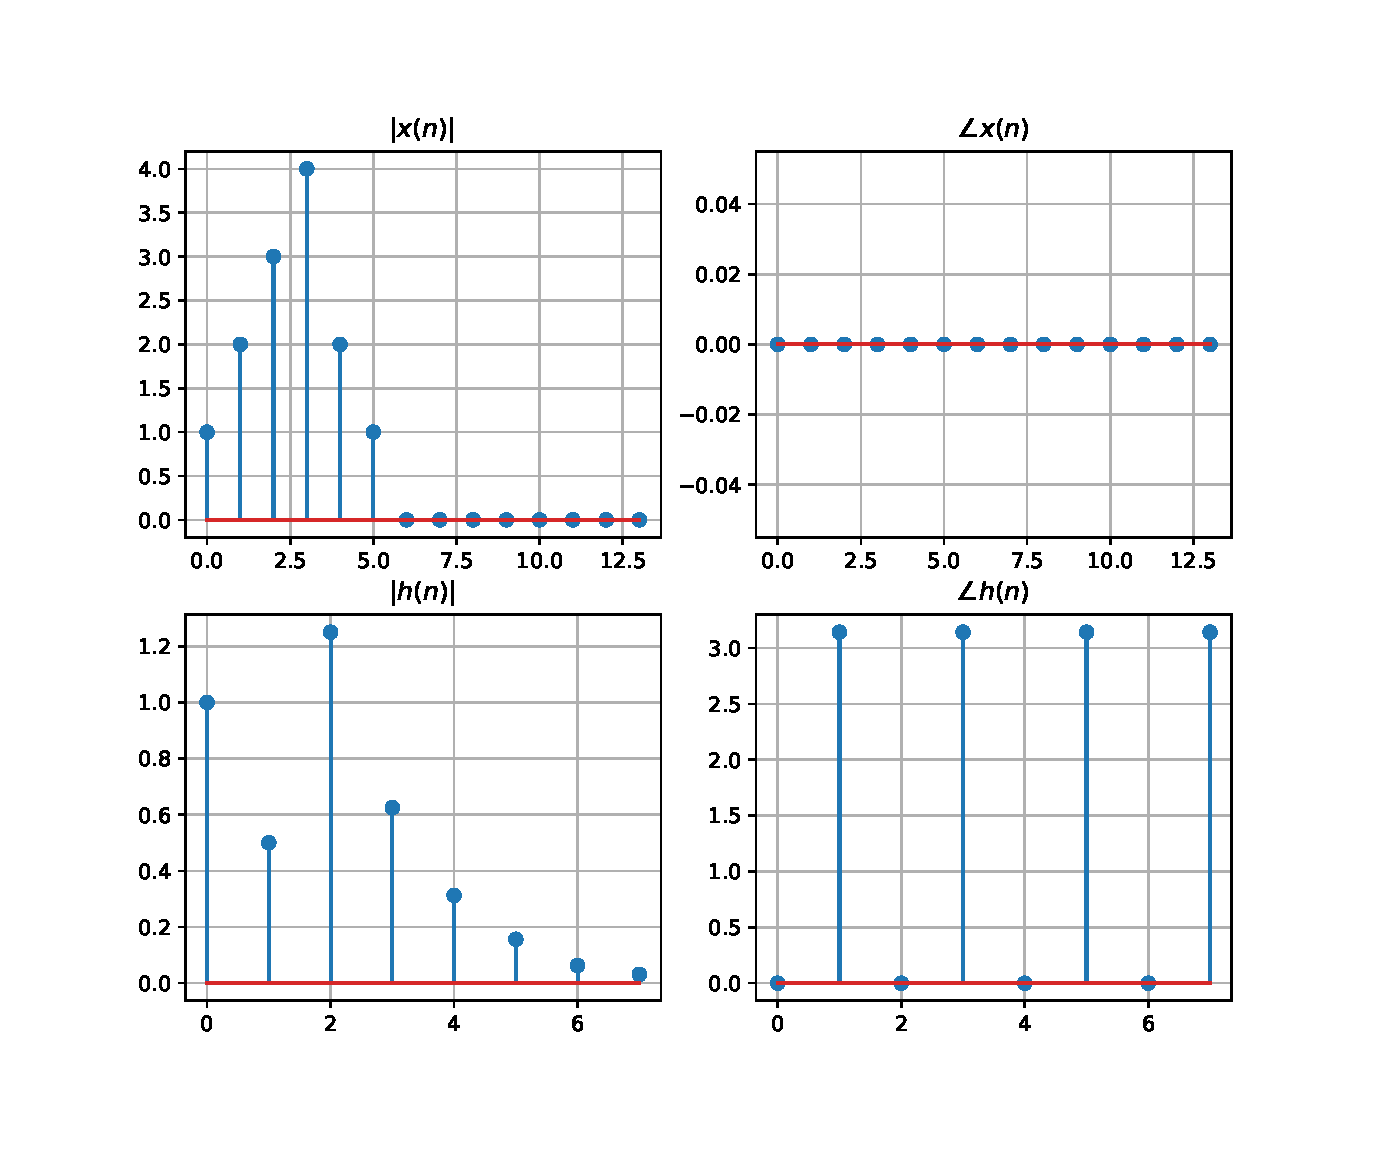
\includegraphics[width=9cm]{./figs/ee18btech11029_1.eps}
    \caption{Input signal x(n) and Impulse response h(n)}
    \label{yn}
\end{figure}
\item Impulse Response of the System is
\begin{align}
    h(n)=\left(-\frac{1}{2}\right)^{n} u(n)+\left(-\frac{1}{2}\right)^{n-2} u(n-2)	
\end{align}
\item FFT of a Input Signal $x(n)$ is 
\begin{align}
    X(k) = \sum_{n=0}^{N-1} x(n) e^{-j 2 \pi k n / N},\quad k=0,1 \ldots N-1
\end{align}
 
\item FFT of a Impulse Response $h(n)$ is 
\begin{align}
    H(k) = \sum_{n=0}^{N-1} h(n) e^{-j 2 \pi k n / N}, \quad k=0,1, \ldots, N-1
\end{align}

\item FFT of output Signal $y(n)$ can be calculated by 
\begin{align}
    Y(k) = X(k)H(k)
\end{align}
\item $y(n)$ can be calculated by doing IFFT for $Y(k)$
\begin{align}
    y(n) = \frac{1}{N}\sum_{n=0}^{N-1}Y(k) e^{j 2 \pi n k / N}, \quad k=0,1, \ldots, N-1
\end{align}
 
\item Plotting  FFT of output signal 
\begin{figure}[h!]
    \centering
    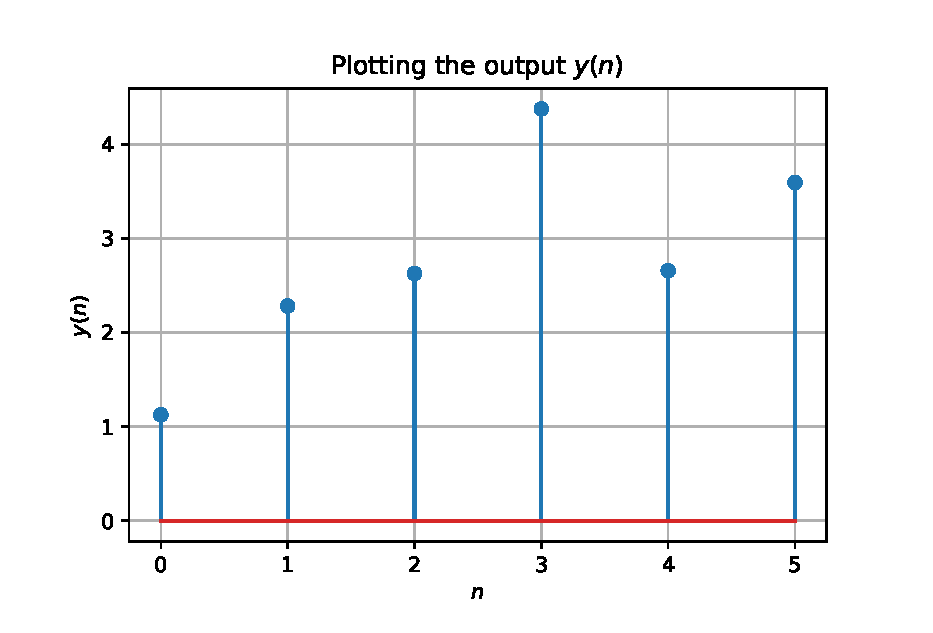
\includegraphics[width=9cm]{./figs/ee18btech11029_2.eps}
    \caption{Output signal $y(n)$}
    \label{YN}
\end{figure}


\end{enumerate}

\section{problem}
\begin{enumerate}[label=\thesection.\arabic*.,ref=\thesection.\theenumi]
    \numberwithin{equation}{enumi}
    \item Wherever possible, express all the above equations as matrix equations.
\end{enumerate}
\section{Solution}
\begin{enumerate}[label=\thesection.\arabic*.,ref=\thesection.\theenumi]
    \numberwithin{equation}{enumi}
    \item FFT of signal X(n) 
    \begin{align}
        X(k) \triangleq \sum_{n=0}^{N-1} x(n) e^{-j 2 \pi k n / N}, \quad k=0,1, \ldots, N-1
    \end{align}
    \item Let $W_{N}^{n k}=e^{-j 2 \pi k n / N}$ then this can be $\mathrm{ex}-$ pressed interms of matrices as:
    \begin{align}
        \begin{bmatrix} X(0) \\ X(1) \\ X(2) \\ X(3) \\ X(4) \\ X(5) \end{bmatrix}
=
\begin{bmatrix}
1 & 1 & 1 & 1 & 1 & 1 \\ 1 & W_N^1& W_N^2& W_N^3 & W_N^4 & W_N^5\\1 & W_N^2 & W_N^4 & W_N^6 & W_N^8 & W_N^{10}\\1 & W_N^3 & W_N^6 & W_N^9 & W_N^{12} & W_N^{15}\\1 & W_N^4 & W_N^8 & W_N^{12} & W_N^{16} & W_N^{20}\\1 & W_N^5 & W_N^{10} & W_N^{15} & W_N^{20} &W_N^{25}
\end{bmatrix}%
\begin{bmatrix}
x(0) \\ x(1) \\ x(2) \\ x(3) \\ x(4) \\x(5)
\end{bmatrix}
    \end{align}
 \item Given that $x(n)=\{1,2,3,4,2,1\}$
and $\mathrm{As}, \mathrm{N}=6$ then above equation on multiplying matrices becomes
\begin{align}
    \begin{bmatrix} X(0) \\ X(1) \\ X(2) \\ X(3) \\ X(4) \\ X(5) \end{bmatrix}
=
\begin{bmatrix}
1 +2+3+4+2+1 \\ 1+ (2)e^{-j\pi /3} + ... + (1)e^{-j5\pi /3}\\ 1 + (2)e^{-2j\pi /3} + ... +(1)(e^{-2j5\pi /3}\\ 1 + (2)e^{-3j\pi /3} + ... + (1)e^{-3j5\pi /3}\\ 1 + (2)e^{-4j\pi /3} + ... + (1)e^{-4j5\pi /3}\\ 1 + (2)e^{-5j\pi /3} + ... + (1)e^{-5j5\pi /3}
\end{bmatrix}
\end{align}
\item
On solving we get,
\begin{align}
    \begin{bmatrix} X(0) \\ X(1) \\ X(2) \\ X(3) \\ X(4) \\ X(5) \end{bmatrix}
=
\begin{bmatrix}
13 \\ 
-4-\sqrt{3}j\\ 
1  \\ 
-1 \\ 
1 \\ 
-4+\sqrt{3}j
\end{bmatrix}
\end{align}
\begin{align}
    \implies X(0) = 13 + 0j,\\
    X(1) = -4 - 1.732j,\\
    X(2) = 1 + 0j,
    \\
    X(3) = -1 + 0j,\\
    X(4) = 1 + 0j,\\
    X(5) = -4 + 1.732j
\end{align}
\begin{figure}[h!]
    \centering
    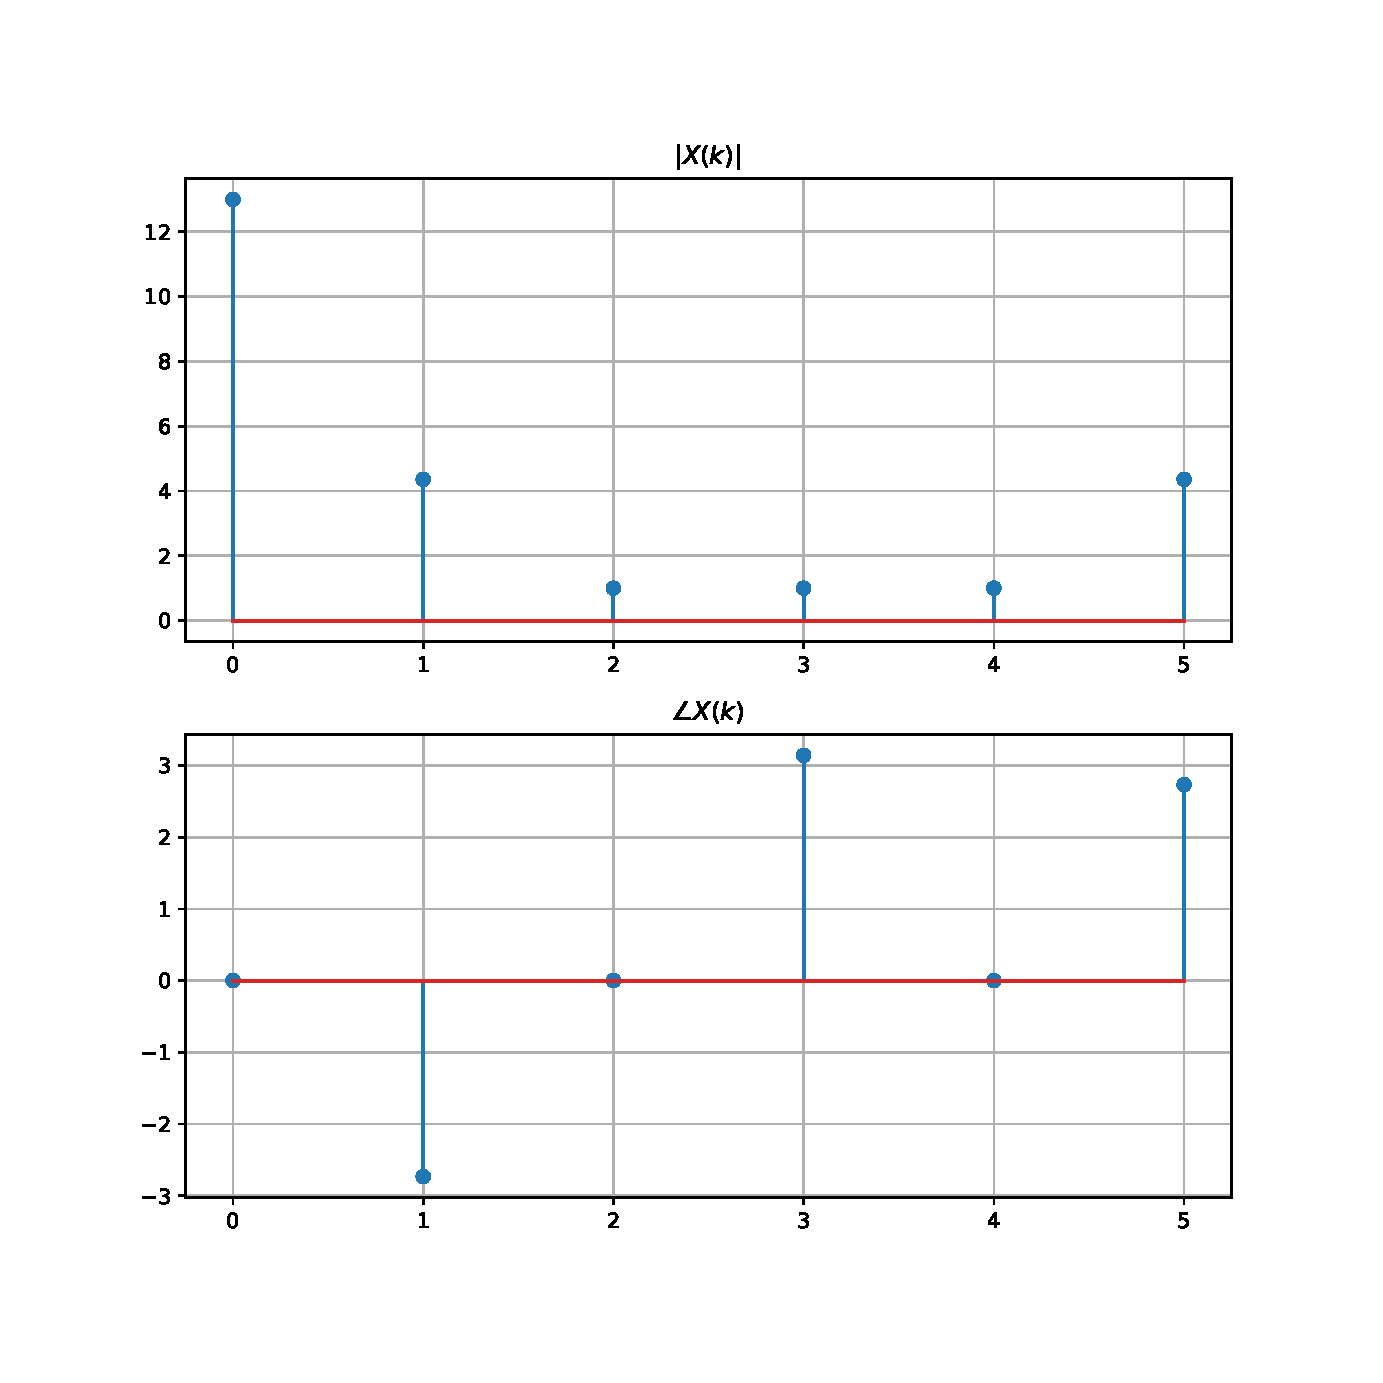
\includegraphics[width=9cm]{./figs/ee18btech11029_3.eps}
    \caption{FFT of $x(n)$}
    \label{yn}
\end{figure}
\item
Now to find $H(k)$ we need to know the h(n).For that we need to first find the Y(z) by applying Z-transform on equation i.e.,
\begin{align}
    Y(z) + \frac{1}{2}z^{-1}Y(z)=X(z) + z^{-2}X(z)
\end{align}
\begin{align}
    \implies Y(z)=\frac{2(z^2+1)}{z(2z+1)}X(z)
\end{align}
\
Now we can find H(z) using Y(z)\\
 i.e.,
\begin{align}
    H(z) = \frac{Y(z)}{X(z)}
\end{align}
\begin{align}
 H(z) = \frac{2(z^2+1)}{z(2z+1)}
\end{align}
\begin{align}
 H(z) = \frac{1+z^{-2}}{1+\frac{1}{2}z^{-1}}
\end{align}
By applying inverse Z - transform we can find the value of $h(n)$
\begin{align}
 h(n)= Z^{-1}\sbrak{\frac{1}{1+\frac{1}{2}z^{-1}} + \frac{z^{-2}}{1+\frac{1}{2}z^{-1}}}
\end{align}
\begin{align}
 h(n)=\sbrak{\frac{-1}{2}}^nu(n) + \sbrak{\frac{-1}{2}}^{n-2}u(n-2)
\end{align}
\
 Assuming that length of h(n) is same as length of x(n) i.e., N = 6.
Now finding the value of $h(n)$ using matrix method we get

\begin{align}
    \begin{bmatrix} 
H(0) \\ 
H(1) \\ 
H(2) \\ 
H(3) \\ 
H(4) \\ 
H(5) 
\end{bmatrix}
=
\begin{bmatrix}
1 & 1 & 1 & 1 & 1 & 1 \\ 1 & W_N^1& W_N^2& W_N^3 & W_N^4 & W_N^5\\1 & W_N^2 & W_N^4 & W_N^6 & W_N^8 & W_N^{10}\\1 & W_N^3 & W_N^6 & W_N^9 & W_N^{12} & W_N^{15}\\1 & W_N^4 & W_N^8 & W_N^{12} & W_N^{16} & W_N^{20}\\1 & W_N^5 & W_N^{10} & W_N^{15} & W_N^{20} &W_N^{25}
\end{bmatrix}%
\begin{bmatrix}
h(0) \\ 
h(1) \\ 
h(2) \\ 
h(3) \\ 
h(4) \\ 
h(5)
\end{bmatrix}
\end{align}
$
\begin{bmatrix} 
H(0) \\ 
H(1) \\ 
H(2) \\ 
H(3) \\ 
H(4) \\ 
H(5) 
\end{bmatrix}
$
$=$
$
\begin{bmatrix}
h(0) + h(1) + h(2) + h(3) + h(4) + h(5) \\
h(0) + h(1)e^{-j\pi /3} + ... + h(5)e^{-j5\pi /3}\\
h(0) + h(1)e^{-2j\pi /3} + ... + h(5)e^{-2j5\pi /3}\\
h(0) + h(1)e^{-3j\pi /3} + ... + h(5)e^{-3j5\pi /3}\\
h(0) + h(1)e^{-4j\pi /3} + ... + h(5)e^{-4j5\pi /3}\\
h(0) + h(1)e^{-5j\pi /3} + ... + h(5)e^{-5j5\pi /3}
\end{bmatrix}
\\
$
\item
On solving we get\\
\begin{align}
\begin{bmatrix} 
H(0) \\ 
H(1) \\ 
H(2) \\ 
H(3) \\ 
H(4) \\ 
H(5) 
\end{bmatrix}
=
\begin{bmatrix}
1.28125 \\
0.51625-0.5142j \\ 
-0.07813+1.1096j  \\ 
3.84375 \\ 
-0.07183-1.1096j \\ 
0.51625+0.5142j
\end{bmatrix}
\end{align}
\begin{align}
\implies H(0) = 1.28125 + 0j,\\
 H(1) = 0.51625 - 0.5141875j,\\
 H(2) = -0.078125 + 1.1095625j,\\
 H(3) = 3.84375 + 0j,\\
 H(4) = -0.071825 - 1.1095625j.\\
 H(5) = 0.515625 + 0.5141875j
\end{align}

\begin{figure}[h!]
    \centering
    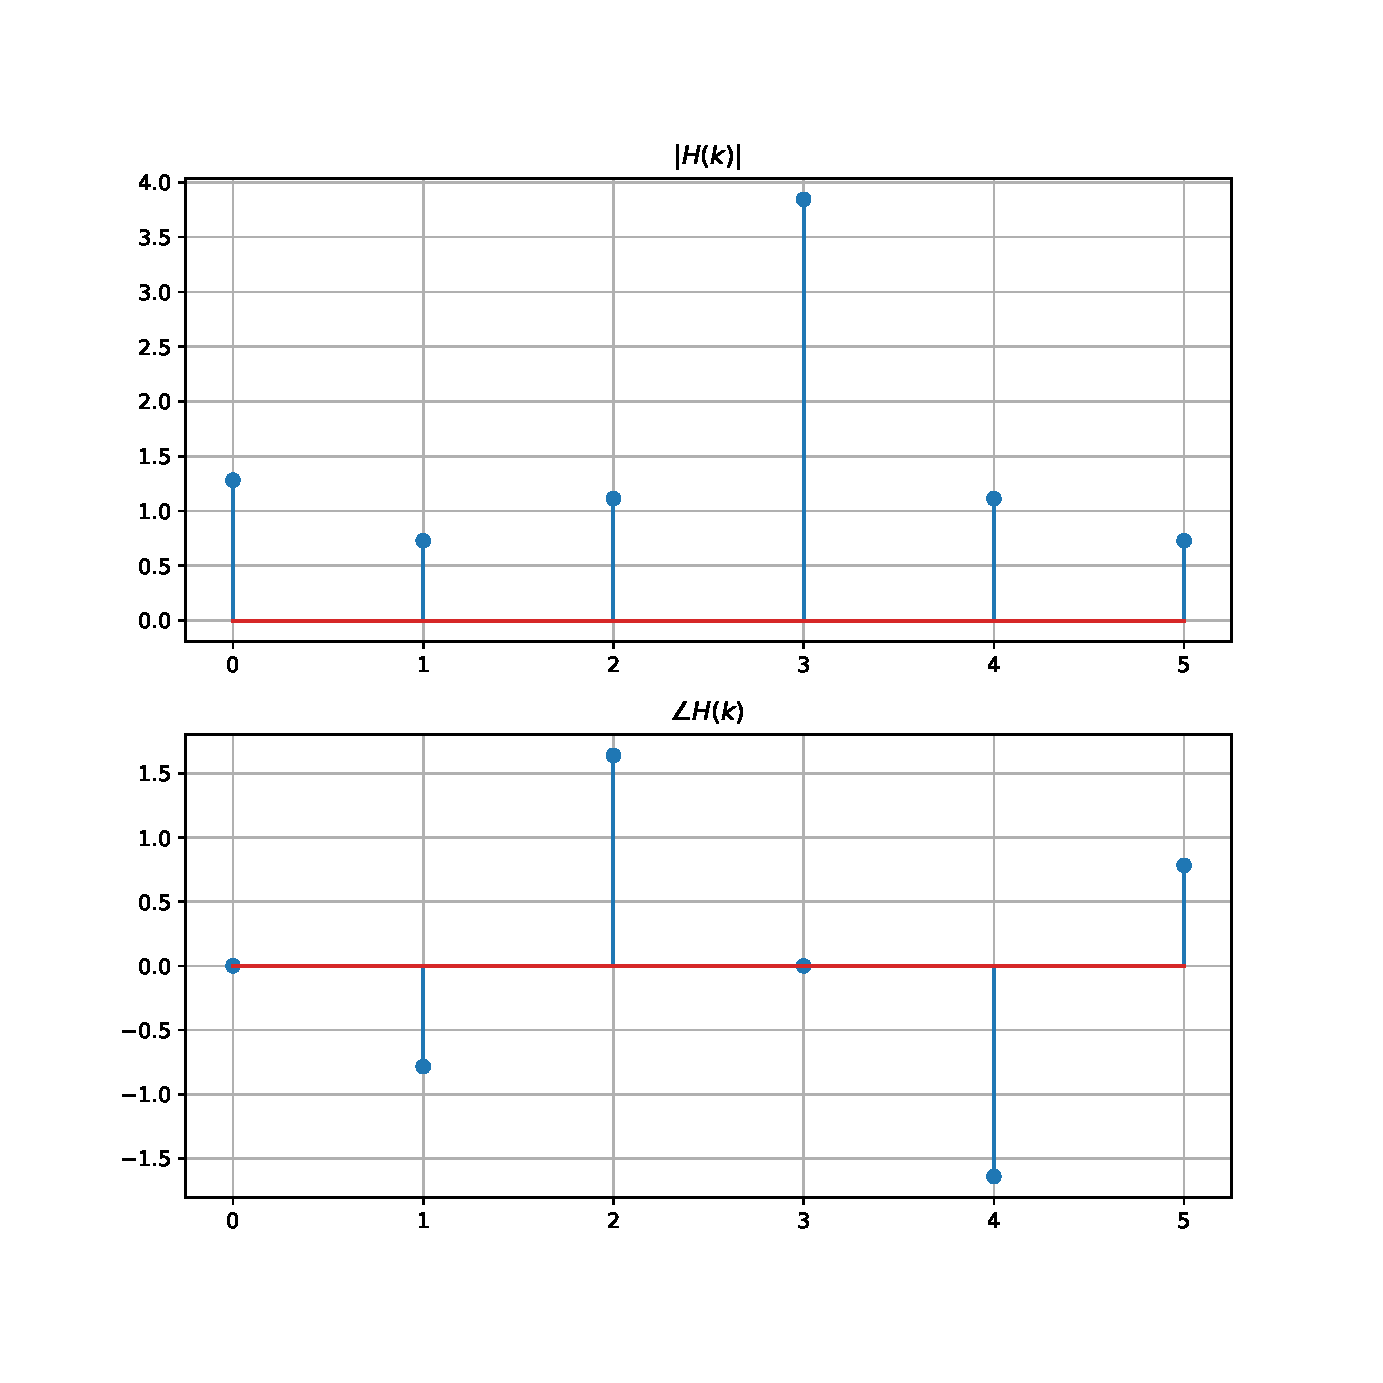
\includegraphics[width=9cm]{./figs/ee18btech11029_4.eps}
    \caption{FFT of $h(n)$}
    \label{yn}
\end{figure}

So,These values which we got are same as that of from the plots.
\item
Now to find $H(k)$ we need to know the h(n).For that we need to first find the Y(z) by applying Z-transform on equation
\begin{equation}
\begin{bmatrix} 
Y(0) \\ 
Y(1) \\ 
Y(2) \\ 
Y(3) \\ 
Y(4) \\ 
Y(5) 
\end{bmatrix}
=
\begin{bmatrix} 
X(0) \\ 
X(1) \\ 
X(2) \\ 
X(3) \\ 
X(4) \\ 
X(5) 
\end{bmatrix}
\times
\begin{bmatrix} 
H(0) \\ 
H(1) \\ 
H(2) \\ 
H(3) \\ 
H(4) \\ 
H(5) 
\end{bmatrix}
\end{equation}
\begin{equation}
\begin{bmatrix} 
Y(0) \\ 
Y(1) \\ 
Y(2) \\ 
Y(3) \\ 
Y(4) \\ 
Y(5) 
\end{bmatrix}
=
\begin{bmatrix}
16.65625\\ 
-2.95312+1.16372j \\ 
-0.07813+1.1096j \\ 
-3.84375\\ 
-0.07813-1.1096j \\ 
-2.95312-1.16372j 
\end{bmatrix}
\end{equation}
\begin{figure}[h!]
    \centering
    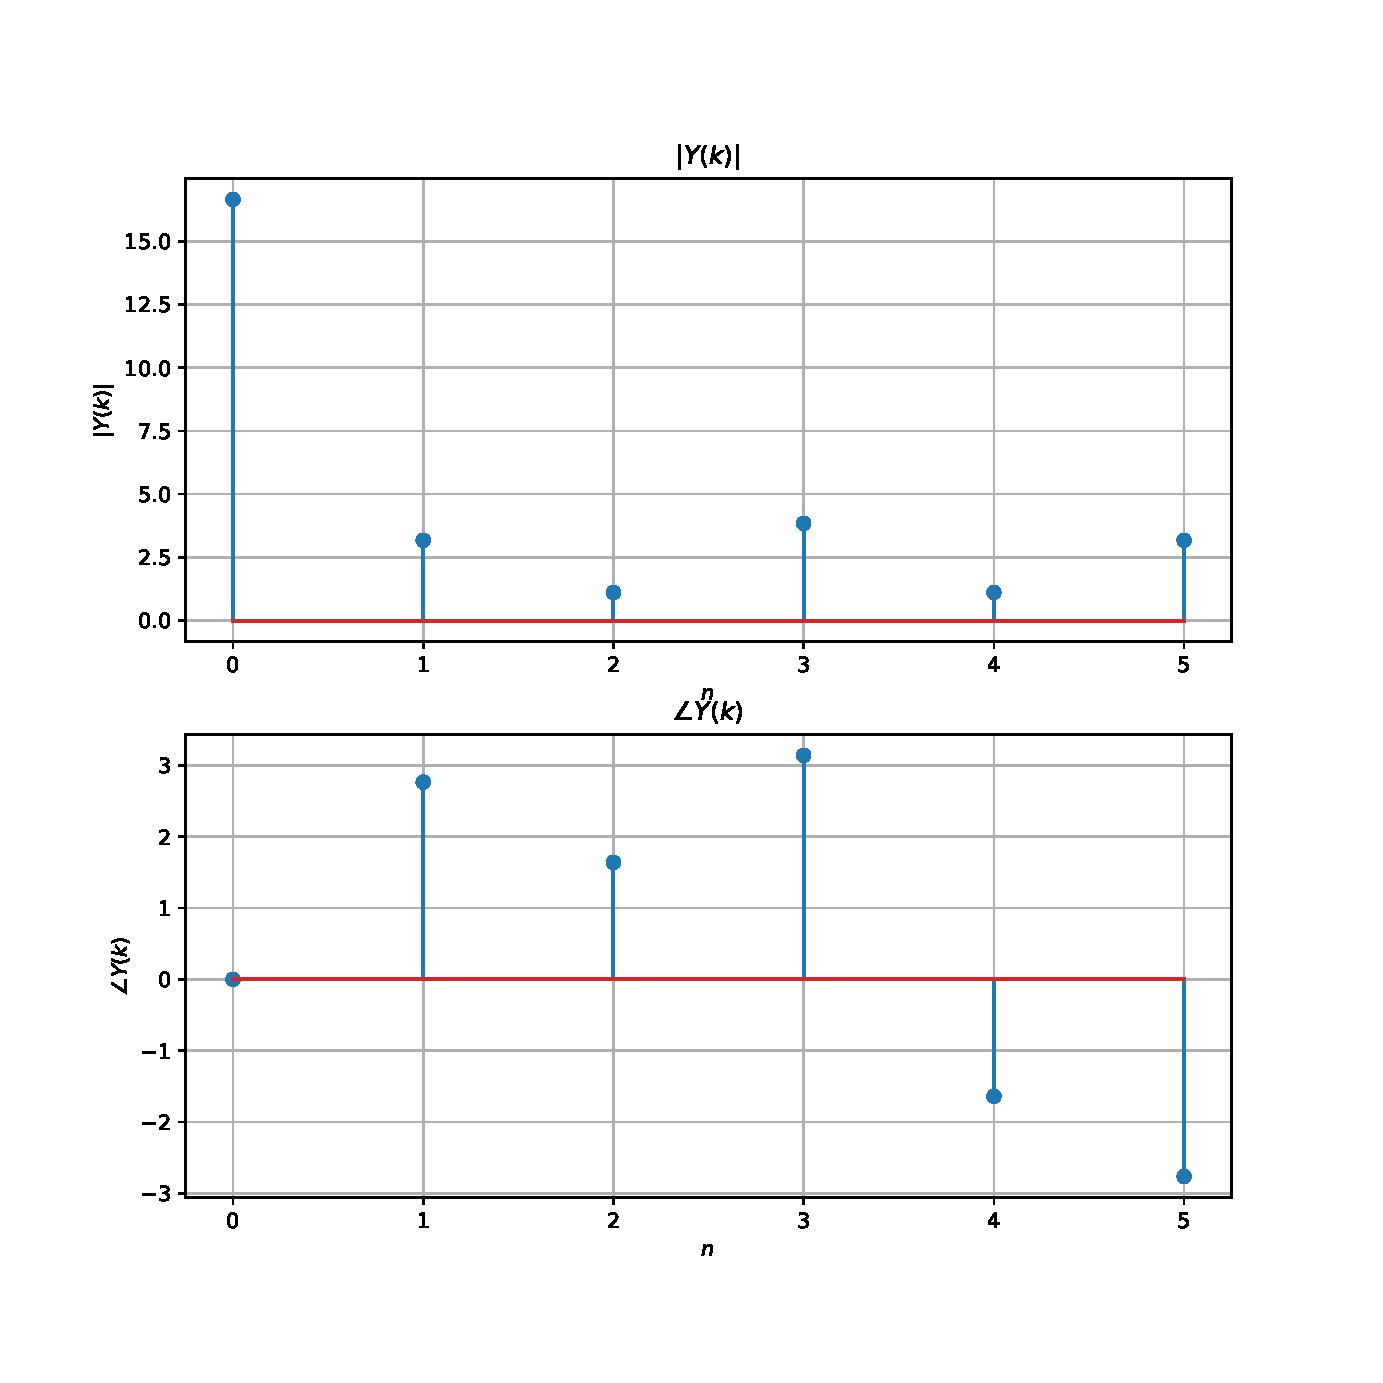
\includegraphics[width=9cm]{./figs/ee18btech11029_5.eps}
    \caption{FFT of $y(n)$}
    \label{yn}
\end{figure}
\item
$y(n)$ can be calculated by applying IFFT for the above Y matrix and is calculated by python code\\
\\
$
\begin{bmatrix} 
y(0) \\ y(1) \\ y(2) \\ y(3) \\ y(4) \\ y(5) 
\end{bmatrix}
=
\begin{bmatrix}
1.125      \\ 2.28125071 \\ 2.6250019 \\ 4.37499667\\ 2.6562481 \\ 3.59375262\\
\end{bmatrix}
\\
\\
$
These are the same values that we have plotted in the above plot \eqref{YN}

\begin{figure}[h!]
    \centering
    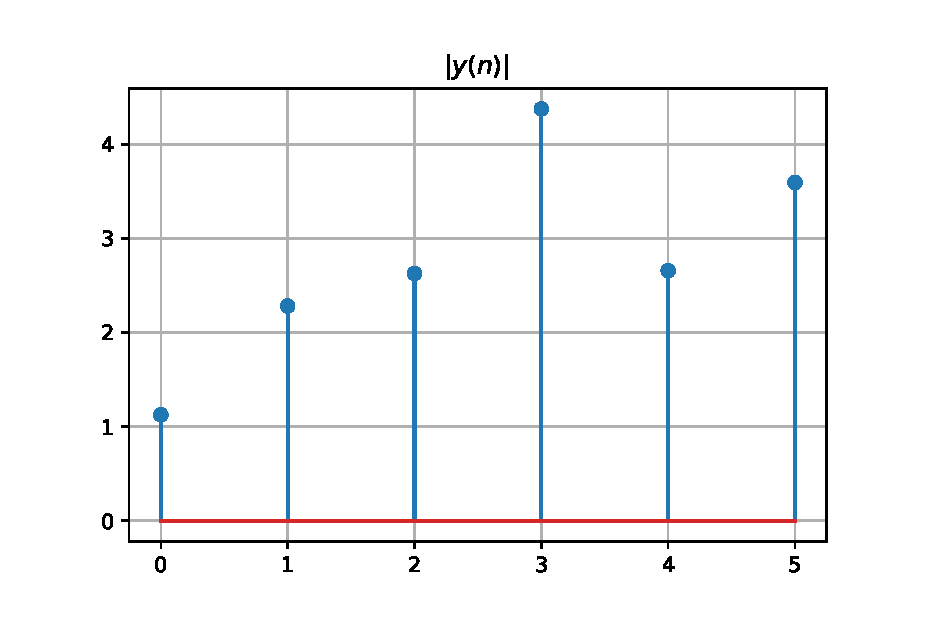
\includegraphics[width=9cm]{./figs/ee18btech11029_6.eps}
    \caption{IFFT of $Y(k)$}
    \label{yn}
\end{figure}
\item
Properties :
\begin{enumerate}
    \item Symmetry property : \[ W^{k+N/2}_{N} = - W^{k}_{N} \] 
    \label{p:p1}
    \item Periodicity property :  \[ W^{k+N}_{N} =  W^{k}_{N} \]     
    \label{p:p2}
    \item \[ W^{2}_{N} =  W_{N/2} \] 
    \label{p:p3}
\end{enumerate}
\item 
Using properties to derive FFT from DFT :
    \begin{align}
       \mathcal X(k) &=  \sum_{n=0}^{N-1} x(n)W^{kn}_{N}, \quad k=0,1, \ldots, N-1 \\
       &= \sum_{n=even} x(n)W^{kn}_{N} + \sum_{n=odd} x(n)W^{kn}_{N} \\
       &= \sum_{m=0}^{2} x(2m)W^{2mk}_{N} + \sum_{m=0}^{2} x(2m+1)W^{(2m+1)k}_{N} 
    \end{align}
using property c, we get,
    \begin{align}
        \mathcal X(k) &= \sum_{m=0}^{2} x(2m)W^{mk}_{N/2} + W^{k}_{N} \sum_{m=0}^{2} x(2m+1)W^{mk}_{N/2} \\
        &= X_{1}(k) + W^{k}_{N}X_{2}(k)
    \end{align}
\item
\begin{itemize}
    \item X\textsubscript{1}(k) and X\textsubscript{2}(k) are 3 point DFTs of x(2m) and x(2m+1) , m=0,1,2.
    \item X\textsubscript{1}(k) and X\textsubscript{2}(k) are periodic, Hence X\textsubscript{1}(k+3) = X\textsubscript{1}(k) and X\textsubscript{2}(k+3) = X\textsubscript{1}(k).
    \item By performing this step once we can see that number of operations have been reduced
    from $N^2$ to $\frac{N^2}{2}$.
\end{itemize}

\item
Let us take  $F_{N}$ as the N-point DFT Matrix. \\
By the property of Complex Exponentials we can write $F_{N}$ in terms of $F_{N/2}$
\begin{equation}
F_{N}=
\begin{bmatrix}
I_{N/2} & D_{N/2} \\
I_{N/2} & -D_{N/2}
\end{bmatrix}
\begin{bmatrix}
F_{N/2} & 0 \\
0 & F_{N/2}
\end{bmatrix}
P_{N}
\end{equation}
For N = 6
\begin{equation}
\implies F_{6}=
\begin{bmatrix}
I_{3} & D_{3} \\
I_{3} & -D_{3}
\end{bmatrix}
\begin{bmatrix}
F_{3} & 0 \\
0 & F_{3}
\end{bmatrix}
P_{6}
\end{equation}
Here
$I_{3}$ is the 3x3 identity matrix. Writing matrices in block form :
\begin{equation}
D_{3}=
\begin{bmatrix}
1 & 0 & 0 \\
0 & W^{1}_{3} & 0 \\
0 & 0 & W^{2}_{3}
\end{bmatrix}
\end{equation}
\begin{equation}
P_{6} =
\begin{bmatrix}
1 & 0 & 0 & 0 & 0 & 0\\
0 & 0 & 1 & 0 & 0 & 0\\
0 & 0 & 0 & 0 & 1 & 0\\
0 & 1 & 0 & 0 & 0 & 0\\
0 & 0 & 0 & 1 & 0 & 0\\
0 & 0 & 0 & 0 & 0 & 1
\end{bmatrix} 
\end{equation}
\begin{equation}
\implies P_{6}
\begin{bmatrix}
x(0) \\ 
x(1) \\ 
x(2) \\ 
x(3) \\ 
x(4) \\ 
x(5)
\end{bmatrix}
= 
\begin{bmatrix}
x(0) \\ 
x(2) \\ 
x(4) \\ 
x(1) \\ 
x(3) \\ 
x(5)
\end{bmatrix}
\end{equation}
Let 
\begin{equation}
\begin{bmatrix}
X_{1}(0) \\ 
X_{1}(1) \\ 
X_{1}(2) 
\end{bmatrix}
= F_{N/2}
\begin{bmatrix}
x(0) \\ 
x(2) \\ 
x(4) \\ 
\end{bmatrix}
\end{equation}
\begin{equation}
\begin{bmatrix}
X_{2}(0) \\ 
X_{2}(1) \\ 
X_{2}(2) 
\end{bmatrix}
= F_{N/2}
\begin{bmatrix}
x(1) \\ 
x(3) \\ 
x(5) \\ 
\end{bmatrix}
\end{equation}
be the N/2 point DFTs.
\item
By replacing the above results in the equation $X = F_{N} x$, we get
\begin{equation}
\begin{bmatrix}
X(0) \\ 
X(1) \\ 
X(2) \\ 
X(3) \\ 
X(4) \\ 
X(5) 
\end{bmatrix}
=
\begin{bmatrix}
1 & 0 & 0 & W^{0}_{6} & 0 & 0\\
0 & 1 & 0 &  0 & W^{1}_{6} & 0\\
0 & 0 & 1 & 0 & 0 & W^{2}_{6}\\
1 & 0 & 0 & -W^{0}_{6} & 0 & 0\\
0 & 1 & 0 & 0 & -W^{1}_{6} & 0\\
0 & 0 & 1 & 0 & 0 & -W^{2}_{6}
\end{bmatrix}
\begin{bmatrix}
X_{1}(0) \\ 
X_{1}(1)\\ 
X_{1}(2)\\ 
X_{2}(0) \\ 
X_{2}(1) \\ 
X_{2}(2)
\end{bmatrix}  
\end{equation}
Using the above method breaking the N-point DFT into two N/2-point DFT's we get
\begin{equation}
\begin{bmatrix}
X(0) \\ 
X(1) \\ 
X(2) \\ 
\end{bmatrix}
=
\begin{bmatrix}
X_{1}(0) \\ 
X_{1}(1)\\ 
X_{1}(2)\\
\end{bmatrix}
+
\begin{bmatrix}
W^{0}_{6} & 0 & 0\\
0 & W^{1}_{6} & 0\\
0 & 0 & W^{2}_{6}\\
\end{bmatrix}
\begin{bmatrix}
X_{2}(0) \\ 
X_{2}(1) \\ 
X_{2}(2)
\end{bmatrix}
\end{equation}
\begin{equation}
\begin{bmatrix}
X(3) \\ 
X(4) \\ 
X(5) 
\end{bmatrix}
=
\begin{bmatrix}
X_{1}(0) \\  
X_{1}(1)\\ 
X_{1}(2)\\
\end{bmatrix}
-
\begin{bmatrix}
W^{0}_{6} & 0 & 0\\
0 & W^{1}_{6} & 0\\
0 & 0 & W^{2}_{6}\\
\end{bmatrix}
\begin{bmatrix}
X_{2}(0) \\ 
X_{2}(1) \\ 
X_{2}(2)
\end{bmatrix} 
\end{equation}
Hence the time complexity is reduced from O($N^{2}$) to O(NlogN). 
\item If we have $N = 2^{M}$ where $M \in \mathbb{Z^{+}}$  then we can recursively breakdown N/2 point DFT Matrix into N/4 point DFT Matrix and so on till we reach 2-point DFT Matrix.\\
for N = 8, we can write,
\begin{equation}
F_{8}=
\begin{bmatrix}
I_{4} & D_{4} \\
I_{4} & -D_{4}
\end{bmatrix}
\begin{bmatrix}
F_{4} & 0 \\
0 & F_{4}
\end{bmatrix}
P_{8}
\end{equation}
\begin{equation}
F_{4}=
\begin{bmatrix}
I_{2} & D_{2} \\
I_{2} & -D_{2}
\end{bmatrix}
\begin{bmatrix}
F_{2} & 0 \\
0 & F_{2}
\end{bmatrix}
P_{4}
\end{equation}
Finally, the 2-point DFT Matrix is the base case 
\begin{equation}
F_{2}
\begin{bmatrix}
x_{1} \\
x_{2}
\end{bmatrix}
=
\begin{bmatrix}
1 & 1 \\
1 & -1
\end{bmatrix}
\begin{bmatrix}
x_{1} \\
x_{2}
\end{bmatrix}
=
\begin{bmatrix}
x_{1}+x_{2} \\
x_{1}-x_{2}
\end{bmatrix}
\end{equation}
\item Step by Step visualization of computing 8-Point DFT recursively using 4-point DFT's and 2-point DFT's.Expressing 8-point DFT's in terms of 4-point DFT's.
\begin{equation}
\begin{bmatrix}
X(0) \\ 
X(1) \\ 
X(2) \\ 
X(3)
\end{bmatrix}
=
\begin{bmatrix}
X_{e}(0) \\ 
X_{e}(1)\\ 
X_{e}(2)\\
X_{e}(3)\\
\end{bmatrix}
+
\begin{bmatrix}
W^{0}_{8} & 0 & 0 & 0\\
0 & W^{1}_{8} & 0 & 0\\
0 & 0 & W^{2}_{8} & 0\\
0 & 0 & 0 & W^{3}_{8}
\end{bmatrix}
\begin{bmatrix}
X_{o}(0) \\ 
X_{o}(1) \\ 
X_{o}(2) \\
X_{o}(3)
\end{bmatrix}
\end{equation}
\begin{equation}
\begin{bmatrix}
X(4) \\ 
X(5) \\ 
X(6) \\ 
X(7)
\end{bmatrix}
=
\begin{bmatrix}
X_{e}(0) \\ 
X_{e}(1)\\ 
X_{e}(2)\\
X_{e}(3)\\
\end{bmatrix}
-
\begin{bmatrix}
W^{0}_{8} & 0 & 0 & 0\\
0 & W^{1}_{8} & 0 & 0\\
0 & 0 & W^{2}_{8} & 0\\
0 & 0 & 0 & W^{3}_{8}
\end{bmatrix}
\begin{bmatrix}
X_{o}(0) \\ 
X_{o}(1) \\ 
X_{o}(2) \\
X_{o}(3)
\end{bmatrix}
\end{equation}
Here representing $X_{e}$ as $X_{1}$ and $X_{o}$ as $X_{2}$\\
4-point FFTs into 2-point FFTs
\begin{equation}
\begin{bmatrix}
X_{1}(0) \\ 
X_{1}(1)\\ 
\end{bmatrix}
=
\begin{bmatrix}
X_{3}(0) \\ 
X_{3}(1)\\ 
\end{bmatrix}
+
\begin{bmatrix}
W^{0}_{4} & 0\\
0 & W^{1}_{4}
\end{bmatrix}
\begin{bmatrix}
X_{4}(0) \\ 
X_{4}(1) \\ 
\end{bmatrix}
\end{equation}
\begin{equation}
\begin{bmatrix}
X_{1}(2) \\ 
X_{1}(3)\\ 
\end{bmatrix}
=
\begin{bmatrix}
X_{3}(0) \\ 
X_{3}(1)\\ 
\end{bmatrix}
-
\begin{bmatrix}
W^{0}_{4} & 0\\
0 & W^{1}_{4}
\end{bmatrix}
\begin{bmatrix}
X_{4}(0) \\ 
X_{4}(1) \\ 
\end{bmatrix}
\end{equation}
\begin{equation}
\begin{bmatrix}
X_{2}(0) \\ 
X_{2}(1)\\ 
\end{bmatrix}
=
\begin{bmatrix}
X_{5}(0) \\ 
X_{5}(1)\\ 
\end{bmatrix}
+
\begin{bmatrix}
W^{0}_{4} & 0\\
0 & W^{1}_{4}
\end{bmatrix}
\begin{bmatrix}
X_{6}(0) \\ 
X_{6}(1) \\ 
\end{bmatrix}
\end{equation}
\begin{equation}
\begin{bmatrix}
X_{2}(2) \\ 
X_{2}(3)\\ 
\end{bmatrix}
=
\begin{bmatrix}
X_{5}(0) \\ 
X_{5}(1)\\ 
\end{bmatrix}
-
\begin{bmatrix}
W^{0}_{4} & 0\\
0 & W^{1}_{4}
\end{bmatrix}
\begin{bmatrix}
X_{6}(0) \\ 
X_{6}(1) \\ 
\end{bmatrix}
\end{equation}
\begin{equation}
P_{8}
\begin{bmatrix}
x(0) \\ 
x(1) \\ 
x(2) \\ 
x(3) \\ 
x(4) \\ 
x(5) \\
x(6) \\
x(7)
\end{bmatrix}
 = 
\begin{bmatrix}
x(0) \\ 
x(2) \\ 
x(4) \\ 
x(6) \\
x(1) \\ 
x(3) \\ 
x(5) \\
x(7)
\end{bmatrix}
\end{equation}
\begin{equation}
P_{4}
\begin{bmatrix}
x(0) \\ 
x(2) \\ 
x(4) \\ 
x(6) \\
\end{bmatrix}
 = 
\begin{bmatrix}
x(0) \\ 
x(4) \\ 
x(2) \\
x(6)
\end{bmatrix}
\end{equation}
\begin{equation}
P_{4}
\begin{bmatrix}
x(1) \\ 
x(3) \\ 
x(5) \\
x(7)
\end{bmatrix}
 = 
\begin{bmatrix}
x(1) \\ 
x(5) \\ 
x(3) \\ 
x(7) \\
\end{bmatrix}
\end{equation}
Therefore,
\begin{equation}
\begin{bmatrix}
X_{3}(0) \\ 
X_{3}(1)\\ 
\end{bmatrix}
= F_{2}
\begin{bmatrix}
x(0) \\ 
x(4) \\ 
\end{bmatrix}
\end{equation}
\begin{equation}
\begin{bmatrix}
X_{4}(0) \\ 
X_{4}(1)\\ 
\end{bmatrix}
= F_{2}
\begin{bmatrix}
x(2) \\ 
x(6) \\ 
\end{bmatrix}
\end{equation}
\begin{equation}
\begin{bmatrix}
X_{5}(0) \\ 
X_{5}(1)\\ 
\end{bmatrix}
= F_{2}
\begin{bmatrix}
x(1) \\ 
x(5) \\ 
\end{bmatrix}
\end{equation}
\begin{equation}
\begin{bmatrix}
X_{6}(0) \\ 
X_{6}(1)\\ 
\end{bmatrix}
= F_{2}
\begin{bmatrix}
x(3) \\ 
x(7) \\ 
\end{bmatrix}
\end{equation}
$X_{3}$ and $X_{4}$ both combined would give $X_{1}$\\
$X_{5}$ and $X_{6}$ both combined would give $X_{2}$ 
\item The following C program will compute and print the FFT (N-point where N is of the form $2^{n}$)
\begin{lstlisting}
https://github.com/saimehar31/EE3025/tree/master/Assignment1/codes/fft.c
\end{lstlisting}
\item Using the above properties recursively we have implemented radix-2 Fast-Fourier transform algorithm.
% \begin{center}
%  \begin{tabular}{||c c c||} 
%  \hline
%  Algorithm & t$(N=128)$ & t$(N=2048)$ \\ [0.5ex] 
%  \hline\hline
%  DTFT & 33.2 ms & 7.36 s \\ 
%  \hline
%  FFT & 1.54 ms & 27.6 ms \\ [1ex] 
%  \hline
% \end{tabular}
% \end{center}
\begin{itemize}
    \item In a N-point DFT matrix multiplication consists of 2$N^{2}$ multiplication so the overall time complexity is in the order of O($N^{2}$)
    \item In FFT we recursively break down each stage into two N/2-point FFT's resulting in logN term and we do this for entire N so combining both we get O(NlogN)
\end{itemize}
\item
Taking an example of 8-point function,
\begin{align}
    x(n) = \cbrak{\underset{\uparrow}{1},2,3,4,2,1,0,0} 
\end{align}
We know that,
\begin{align}
        X(k) \triangleq W_{N}^{nk} x(n), \quad k=0,1, \ldots, N-1
\end{align}
\begin{equation}
\renewcommand{\arraystretch}{1.35}
\setlength\arraycolsep{0.05pt}
\begin{bmatrix}
X(0) \\
X(1) \\
X(2) \\
X(3) \\
X(4) \\
X(5) \\
X(6) \\
X(7)
\end{bmatrix}
=
\begin{bmatrix}
W^{0}_{8} & W^{0}_{8} & W^{0}_{8} & W^{0}_{8} & W^{0}_{8} & W^{0}_{8} & W^{0}_{8} & W^{0}_{8}\\
W^{0}_{8} & W^{1}_{8} & W^{2}_{8} & W^{3}_{8} & W^{4}_{8} & W^{5}_{8} & W^{6}_{8} & W^{7}_{8}\\
W^{0}_{8} & W^{2}_{8} & W^{4}_{8} & W^{6}_{8} & W^{8}_{8} & W^{10}_{8} & W^{12}_{8} & W^{14}_{8}\\
W^{0}_{8} & W^{3}_{8} & W^{6}_{8} & W^{9}_{8} & W^{12}_{8} & W^{15}_{8} & W^{18}_{8} & W^{21}_{8}\\
W^{0}_{8} & W^{4}_{8} & W^{8}_{8} & W^{12}_{8} & W^{16}_{8} & W^{20}_{8} & W^{24}_{8} & W^{28}_{8}\\
W^{0}_{8} & W^{5}_{8} & W^{10}_{8} & W^{15}_{8} & W^{20}_{8} & W^{25}_{8} & W^{30}_{8} & W^{35}_{8}\\
W^{0}_{8} & W^{6}_{8} & W^{12}_{8} & W^{18}_{8} & W^{24}_{8} & W^{30}_{8} & W^{36}_{8} & W^{42}_{8}\\
W^{0}_{8} & W^{7}_{8} & W^{14}_{8} & W^{21}_{8} & W^{28}_{8} & W^{35}_{8} & W^{42}_{8} & W^{49}_{8}
\end{bmatrix}
\begin{bmatrix}
x(0) \\
x(1) \\
x(2) \\
x(3) \\
x(4) \\
x(5) \\
x(6) \\
x(7)
\end{bmatrix}
\end{equation}
\begin{equation}
\renewcommand{\arraystretch}{1.35}
\setlength\arraycolsep{0.05pt}
\begin{bmatrix}
X(0) \\
X(1) \\
X(2) \\
X(3) \\
X(4) \\
X(5) \\
X(6) \\
X(7)
\end{bmatrix}
=
\begin{bmatrix}
W^{0}_{8} & W^{0}_{8} & W^{0}_{8} & W^{0}_{8} & W^{0}_{8} & W^{0}_{8} & W^{0}_{8} & W^{0}_{8}\\
W^{0}_{8} & W^{1}_{8} & W^{2}_{8} & W^{3}_{8} & W^{4}_{8} & W^{5}_{8} & W^{6}_{8} & W^{7}_{8}\\
W^{0}_{8} & W^{2}_{8} & W^{4}_{8} & W^{6}_{8} & W^{8}_{8} & W^{10}_{8} & W^{12}_{8} & W^{14}_{8}\\
W^{0}_{8} & W^{3}_{8} & W^{6}_{8} & W^{9}_{8} & W^{12}_{8} & W^{15}_{8} & W^{18}_{8} & W^{21}_{8}\\
W^{0}_{8} & W^{4}_{8} & W^{8}_{8} & W^{12}_{8} & W^{16}_{8} & W^{20}_{8} & W^{24}_{8} & W^{28}_{8}\\
W^{0}_{8} & W^{5}_{8} & W^{10}_{8} & W^{15}_{8} & W^{20}_{8} & W^{25}_{8} & W^{30}_{8} & W^{35}_{8}\\
W^{0}_{8} & W^{6}_{8} & W^{12}_{8} & W^{18}_{8} & W^{24}_{8} & W^{30}_{8} & W^{36}_{8} & W^{42}_{8}\\
W^{0}_{8} & W^{7}_{8} & W^{14}_{8} & W^{21}_{8} & W^{28}_{8} & W^{35}_{8} & W^{42}_{8} & W^{49}_{8}
\end{bmatrix}
\begin{bmatrix}
1 \\
2 \\
3 \\
4 \\
2 \\
1 \\
0 \\
0
\end{bmatrix}
\end{equation}
\begin{equation}
\implies
\begin{bmatrix}
X(0) \\
X(1) \\
X(2) \\
X(3) \\
X(4) \\
X(5) \\
X(6) \\
X(7)
\end{bmatrix}
=
\begin{bmatrix}
13 \\
-3.121 - 6.535j \\
1j \\
1.121 - 0.535j \\
-1 \\
1.121 + 0.535j \\
-1j \\
-3.121 + 6.535j
\end{bmatrix}
\end{equation}
\begin{equation}
\renewcommand{\arraystretch}{1.35}
\setlength\arraycolsep{0.05pt}
\begin{bmatrix}
H(0) \\
H(1) \\
H(2) \\
H(3) \\
H(4) \\
H(5) \\
H(6) \\
H(7)
\end{bmatrix}
=
\begin{bmatrix}
W^{0}_{8} & W^{0}_{8} & W^{0}_{8} & W^{0}_{8} & W^{0}_{8} & W^{0}_{8} & W^{0}_{8} & W^{0}_{8}\\
W^{0}_{8} & W^{1}_{8} & W^{2}_{8} & W^{3}_{8} & W^{4}_{8} & W^{5}_{8} & W^{6}_{8} & W^{7}_{8}\\
W^{0}_{8} & W^{2}_{8} & W^{4}_{8} & W^{6}_{8} & W^{8}_{8} & W^{10}_{8} & W^{12}_{8} & W^{14}_{8}\\
W^{0}_{8} & W^{3}_{8} & W^{6}_{8} & W^{9}_{8} & W^{12}_{8} & W^{15}_{8} & W^{18}_{8} & W^{21}_{8}\\
W^{0}_{8} & W^{4}_{8} & W^{8}_{8} & W^{12}_{8} & W^{16}_{8} & W^{20}_{8} & W^{24}_{8} & W^{28}_{8}\\
W^{0}_{8} & W^{5}_{8} & W^{10}_{8} & W^{15}_{8} & W^{20}_{8} & W^{25}_{8} & W^{30}_{8} & W^{35}_{8}\\
W^{0}_{8} & W^{6}_{8} & W^{12}_{8} & W^{18}_{8} & W^{24}_{8} & W^{30}_{8} & W^{36}_{8} & W^{42}_{8}\\
W^{0}_{8} & W^{7}_{8} & W^{14}_{8} & W^{21}_{8} & W^{28}_{8} & W^{35}_{8} & W^{42}_{8} & W^{49}_{8}
\end{bmatrix}
\begin{bmatrix}
1 \\
-0.5 \\
1.25 \\
-0.65 \\
0.3125 \\
-0.15625 \\
0.078125 \\
-0.0390625
\end{bmatrix}
\end{equation}
\begin{equation}
\implies
\begin{bmatrix}
H(0) \\
H(1) \\
H(2) \\
H(3) \\
H(4) \\
H(5) \\
H(6) \\
H(7)
\end{bmatrix}
=
\begin{bmatrix}
1.32 \\
0.858 - 0.514j \\
-0.015-0.007j \\
0.516 +1.829j \\
3.96 \\
0.516 - 1.829j \\
-0.015+0.007j  \\
0.858 + 0.514j
\end{bmatrix}
\end{equation}
So,
\begin{equation}
\begin{bmatrix} 
Y(0) \\ Y(1) \\ Y(2) \\ Y(3) \\ Y(4) \\ Y(5) \\ Y(6) \\ Y(7) 
\end{bmatrix}
=
\begin{bmatrix}
X(0)\cdot H(0) \\ X(1)\cdot H(1) \\ X(2)\cdot H(2) \\ X(3)\cdot H(3) \\ X(4)\cdot H(4) \\ X(5)\cdot H(5) \\ X(6)\cdot H(6) \\ X(7)\cdot H(7)
\end{bmatrix}
\end{equation}
Solving,
\begin{equation}
\implies
\begin{bmatrix}
Y(0) \\
Y(1) \\
Y(2) \\
Y(3) \\
Y(4) \\
Y(5) \\
Y(6) \\
Y(7)
\end{bmatrix}
=
\begin{bmatrix}
17.16 \\
-6.04 - 4j \\
-0.007-0.015j \\
1.55 +1.77j \\
-3.96 \\
1.55 -1.77j\\
0.007+0.015j  \\
-6.04 + 4j
\end{bmatrix}
\end{equation}
Similary we get
\begin{equation}
\begin{bmatrix}
y(0) \\
y(1) \\
y(2) \\
y(3) \\
y(4) \\
y(5) \\
y(6) \\
y(7)
\end{bmatrix}
=
\begin{bmatrix}
0.53125 \\
1.69 \\
3.09 \\
4.375 \\
2.773\\
3.593\\
0.203\\
0.8984
\end{bmatrix}
\end{equation}
\end{enumerate}
\end{document}


